%%%%%%%%%%%%%%%%%%%%%%%%%%%%%%%%%%%%%%%%%
% Journal Article
% LaTeX Template
% Version 1.0 (25/8/12)
%
% This template has been downloaded from:
% http://www.LaTeXTemplates.com
%
% Original author:
% Frits Wenneker (http://www.howtotex.com)
%
% License:
% CC BY-NC-SA 3.0 (http://creativecommons.org/licenses/by-nc-sa/3.0/)
%
%%%%%%%%%%%%%%%%%%%%%%%%%%%%%%%%%%%%%%%%%

%----------------------------------------------------------------------------------------
%	PACKAGES AND OTHER DOCUMENT CONFIGURATIONS
%----------------------------------------------------------------------------------------

\documentclass[twoside]{article}

\usepackage{lipsum} % Package to generate dummy text throughout this template

\usepackage[sc]{mathpazo} % Use the Palatino font
\usepackage[T1]{fontenc} % Use 8-bit encoding that has 256 glyphs
\linespread{1.05} % Line spacing - Palatino needs more space between lines
\usepackage{microtype} % Slightly tweak font spacing for aesthetics

\usepackage[hmarginratio=1:1,top=32mm,columnsep=20pt]{geometry} % Document margins
\usepackage{multicol} % Used for the two-column layout of the document
\usepackage{hyperref} % For hyperlinks in the PDF

\usepackage[hang, small,labelfont=bf,up,textfont=it,up]{caption} % Custom captions under/above floats in tables or figures
\usepackage{booktabs} % Horizontal rules in tables
\usepackage{float} % Required for tables and figures in the multi-column environment - they need to be placed in specific locations with the [H] (e.g. \begin{table}[H])

\usepackage{graphicx}
\usepackage{amsmath} 
\usepackage{caption}
\usepackage{epsfig}
\usepackage{subcaption}
\usepackage{lettrine} % The lettrine is the first enlarged letter at the beginning of the text
\usepackage{paralist} % Used for the compactitem environment which makes bullet points with less space between them

\usepackage{abstract} % Allows abstract customization
\renewcommand{\abstractnamefont}{\normalfont\bfseries} % Set the "Abstract" text to bold
\renewcommand{\abstracttextfont}{\normalfont\small\itshape} % Set the abstract itself to small italic text

\usepackage{titlesec} % Allows customization of titles
%\titleformat{\section}[block]{\large\scshape\centering{\Roman{section}.}}{}{1em}{} % Change the look of the section titles 

\usepackage{fancyhdr} % Headers and footers
\pagestyle{fancy} % All pages have headers and footers
\fancyhead{} % Blank out the default header
\fancyfoot{} % Blank out the default footer
\fancyhead[C]{Astronomy 330 : Paper 2} % Custom header text
\fancyfoot[RO,LE]{\thepage} % Custom footer text

%-----New Commands


%----------------------------------------------------------------------------------------
%	TITLE SECTION
%----------------------------------------------------------------------------------------

\title{\vspace{-15mm}\fontsize{24pt}{10pt}\selectfont\textbf{Exploring the Cosmological Constant}} % Article title

\author{
\large
\textsc{Allan Gamboa}\\ % Your name
\normalsize San Francisco State University
\vspace{-5mm}
}
\date{}

%=========================================
%=========================================
\begin{document}

\maketitle % Insert title

\thispagestyle{fancy} % All pages have headers and footers
%=========================================
%=========================================


\section{Introduction}
Before Hubble's ground breaking discovery in 1929 where he identified a relationship between a Galaxy's' distance and its radial velocity, there was no reason to discredit a static universe. In fact around the when Albert Einstein first published his theory of General Relativity, the scientific society was not sure that galaxies outside our own existed. There appeared to be just as many stars and fuzzy patches moving towards us as there where moving away from us leading the community of the time to believe that we in fact lived in a static universe. The problem with this notion though is that Einstein's theory made such a universe science fiction.\par
In an effort to avoid the complexity of Einsteins field equations I will follow a discussion given in \emph{Introduction to Cosmology} by Barbara Ryden,  the concern is nicely illustrated through the use of Newtoniain theory. From Possion's equation for gravity.
\begin{align}
\nabla^{2}\Phi = 4\pi G\rho\label{eq:poisson}
\end{align} 
where $\Phi$ is the gravitational potential, $G$ is the well known and appreciated gravitational constant, and rho is the mass density of the universe. Now noting that the force is the gradient of the potential implying that acceleration is proportional to the gradient ($\nabla\Phi = -\ddot{\vec{x}}$, here the acceleration is denoted by $\ddot{\vec{x}}$) we see that a static universe(i.e. $\dot{\vec{x}}=\ddot{\vec{x}} = 0$) only if,
\begin{align}
\rho = \frac{1}{4\pi G}\nabla^{2}\Phi = 0
\end{align}
This is a universe completely void of matter
%----------------------------------
\footnote{From $E=mc^{2}$ also completely void of energy.},
%----------------------------------
one merely needs to look up to see that this is not the case!\par

However if one introduces a term, ad hoc, to equation~\ref{eq:poisson} such that,
\begin{align}
\nabla^{2}\Phi + \Lambda = 4\pi G\rho
\end{align}
a static universe is completely acceptable, since with this formulation it does not directly imply an empty one.

%==================================
\subsection{The Friedmann Equation}\label{s:friedCurv}
%==================================

The Newtonian analysis is but an approximation to general relativity. In order to understand the full implications of the cosmological constant one must invoke the Friedmann equation, derived from the Einsteins field equations for gravity. With the inclusion of the cosmological constant it takes the following form
\begin{align}
\left(\frac{\dot{a}(t)}{a(t)}\right)^{2} = \frac{8\pi G}{3}\rho(t)-\frac{kc^{2}}{a^{2}(t)} + \frac{\Lambda}{3}\label{eq:fried}
\end{align}
Here $a$ is the scale factor, it represents the amount the universe has grown. Positions in the universe are defined by both a comoving coordinate and the scale factor ($r(t) = r_{c}a(t)$). We note that all the time dependence is locked in $a$. The scale factor essentially encapsulates the dynamical history of the universe and predicts its future; it is normalized to be one now ($t=t_{0}$) and 0 at $t=0$ for a big bang universe. $k$ is the curvature constant which defines the geometrical topology of the universe. Table~\ref{t:curvature} introduces the relevance of this parameter. $\Lambda$ is Einsteins Cosmological constant which, today, has been defined to be proportional to the density of Dark Energy in the universe.   $\rho$ is the density of the universe due to anything other than $\Lambda$.

\begin{table}[h!]
  \begin{center}
    \begin{tabular}{ r | l }
    \hline\hline
    $\boldsymbol{$k$}$ & \textbf{Physical Significance}   \\\hline\hline
    0 & This is a flat or euclidian universe also known as an \emph{Einstein de Sitter} universe.\\& In such a universe the angles of a triangle add up to precisely $180^{\circ}$.\\\hline
    >0 & This is commonly referred to as a closed universe. A common closed geometrical\\& shape is a sphere. In such a universe the angles of a triangle add up to a value\\& greater than $180^{\circ}$.\\\hline
    <0 & This is commonly referred to as an open universe. A common open geometrical\\& shape is the surface of a saddle. In such a universe the angles of a triangle add\\& up to a value less than $180^{\circ}$. \\
    \hline
    \end{tabular}
  \end{center}
  \caption{A simple breakdown of the curvture constant}\label{t:curvature}
\end{table}
It is essential to note that the examples referring to 2 dimensional surfaces are not directly applicable. The curvature is a measure of the full 3 dimensional  space not some 2 dimensional subspace. The implications of the curvature constant along with the Cosmological constant will be further explored in the body of the text\footnote{We will be neglecting contributions from matter and readiation to the total density $\rho$.}.

\subsection{The Hubble Parameter}
In 1927 Edwin Hubble declared to the world, through his publication,  that all Galaxies not gravitationally influenced by our own or local group are moving away from us with some velocity proportional to their distance from us. The famous figure depicting this remarkable result is shown on figure~\ref{f:Hubble}. From the plot the slope is approximately $500 [\frac{km}{s\cdot Mpc}]$.  The slope of this plot is referred to as the \emph{Hubble Parameter}, $H(t)$, and it is time dependent. Hubble's  preliminary measurement of his own constant was a grave overestimate due to biasing of galactic distances towards smaller distances.The accepted value of the Hubble parameter today is $H_{0} \approx 72 [\frac{km}{s\cdot Mpc}]$; we note the difference between $H(t)$ and $H_{0}$, where $H_{0} = H(t_{0}) = H(t=today)$, here I hope it is apparent that $t_{0}$ denotes the time today or the time since the big bang. The nice thing about this parameter is that it is easily and directly measurable.\par
We mentioned that the Hubble Parameter is time dependent. In fact it is a measure of how quickly the universe is changing, this is also true of the time derivative of the scale factor and it is not difficult to show (see equation 5.4 in Liddle) that,
\begin{align}
H(t) = \frac{\dot{a}(t)}{a(t)}
\end{align}
This relation becomes useful when trying to simplify the Friedmann equation and express it in totality by observable quantities.

\begin{figure}[h!]
  \centering
      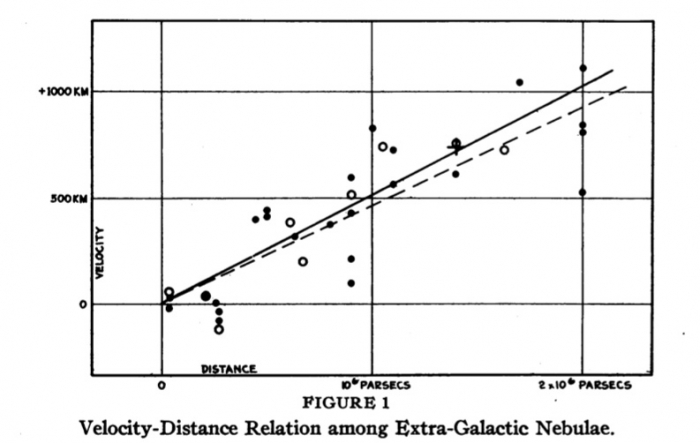
\includegraphics[width=1\textwidth]{hubbleslaw_plot.jpg}
  \caption{Hubbles origional plot depicting the relation  between a galaxies resesional velocity and its distance from us. One notes that he has mislable his $y$ axis to have units of $[km]$ when they should have units of veocity not distance i.e. $[km/s]$ }
\end{figure} 



%=======================================
\section{Simplifying Friedmann's Equation}\label{s:simplify}
%=======================================

The Friedmann equation (eq.~\ref{eq:fried}) takes a particularly useful form  when one considers the \textbf{ Critical Density} which is the density for a flat (i.e. $k=0$) universe. Substituting zero for k,
\begin{align}
&H^{2}(t)=\left(\frac{\dot{a}(t)}{a(t)}\right)^{2} = \frac{8\pi G}{3}\rho(t)+ \frac{\Lambda}{3}\\
&\text{Defining: $\rho_{\Lambda} = \frac{\Lambda}{8\pi G}$ \quad \&\quad  $\rho_{c} = \rho_{\Lambda}+\rho$}\\
&\text{We see that: }\qquad  \rho_{c} = \frac{3H^{2}}{8\pi G}\label{eq:cirtDen}
\end{align}
$\rho_{c}$ is the \emph{Critical Density}.\par

With the critical density in hand we can proceed to express the Friedmann equation in terms of dimensionless parameters. In our analysis we are only concerned with the cosmological parameter ($\Lambda$) and curvature, we may thus express the Friedmann equation as,
\begin{align}
& H^{2}(t) = \frac{8\pi G}{3}\rho_{\Lambda}-\frac{kc^{2}}{a^{2}(t)},\quad \text{Dividing both sides by $\rho_{c}$} \\
&\Longrightarrow 1 = \frac{\rho_{\Lambda}}{\rho_{c}} -\frac{kc^{2}}{a^{2}(t)\rho_{c}},\quad \text{Making the following definitions,}\\
&\Omega_{\Lambda}(t) = \frac{\rho_{\Lambda}}{\rho_{c}} = \rho_{\Lambda}\frac{8\pi G}{3H^{2}}\quad\&\quad\Omega_{k} (t)= -\frac{kc^{2}}{a^{2}\rho_{c}} = -\frac{kc^{2}}{a^{2}}\frac{8\pi G}{3H^{2}}\label{eq:omegasDef}\\
 & \text{We find that the Friedmann equation takes the following form,}\notag\\\notag\\
&\hspace{3.5cm} 1=\Omega_{\Lambda}(t)+\Omega_{k}(t) 
\end{align}\label{eq:friedmanN}
There are a few important points to note about the Friedmann equation in this form. 
\begin{itemize}
\item The $\Omega$'s are dimensionless.
\item Although $\rho_{\Lambda}$ is a constant (i.e. independent of time) $\Omega_{\Lambda}(t)$ is not due to the fact that the critical density, $\rho_{c}$, is dependent on time. 
\item The sum of the $\Omega$'s is always 1, FOR ALL TIME!
\end{itemize}
It would behove us to express the Friedmann equation in terms of quantities we can observe to today (i.e. $t=t_{0}$). First noting that $H_{0} = H(t_{0})$ and $a(t_{0}) = 1$ , It is not difficult to see from equation~\ref{eq:omegasDef} that if we multiply  the top and bottom of both $\Omega_{\Lambda}$ and $\Omega_{k}$ by $H_{0}$ we arrive to the conclusion that, 
\begin{align}
&\Omega_{\Lambda} = \Omega_{\Lambda}(t_{0})\frac{H^{2}_{0}}{H^{2}} = \Omega_{\Lambda,0}\frac{H^{2}_{0}}{H^{2}}\label{eq:omegLamb1}\\
&\Omega_{k} = \frac{\Omega_{k,0}}{a^2}\frac{H_{0}}{H^{2}}
\end{align}
Further by exploiting the third bullet point above we see that $\Omega_{k,0} = 1-\Omega_{\Lambda,0}$, allowing us to express the Friedmann equation (eq~\ref{eq:friedmanN}) as,
\begin{align}
H^2(t) = H^{2}_{0}\left[\Omega_{\Lambda,0}+\frac{1}{a^{2}(t)}(1-\Omega_{\Lambda,0})\right]\label{eq:fried3}
\end{align}



%================================
\section{The Curvature Constant}
%================================
 In section~\ref{s:friedCurv} we introduced the curvature constant $k$ and attempted to provide some conceptual  backing in table~\ref{t:curvature}. As a constant it is time independent and its sign indicates the type of universe we live in. By reinserting $\Omega_{k}$ into equation~\ref{eq:fried3} we can solve for $k$ explicitly arriving to,
\begin{align}
k = \frac{3a^{2}}{8\pi Gc^{2}}(\Omega_{\Lambda,0}H^{2}_{0}-H^{2})
\end{align} 
Because $k$ must remain a constant we can evaluate the expression above for $t=t_{0}$ to arrive to the value of $k$ for all of time.
\begin{align}
k = \frac{3H_{0}^{2}}{8\pi Gc^{2}}(\Omega_{\Lambda,0}-1)\label{eq:OmegaVsK}
\end{align} 
$3H_{0}^{2}/(8\pi Gc^{2})$ must be positive, all the information regarding the sign of $k$ is held in the second term within the parentheses.  The following table, table~\ref{t:signK}, outlines the relationship between $\Omega_{\Lambda,0}$ and $k$.


\begin{table}[h!]
  \begin{center}
    \begin{tabular}{ r| c c }
    \hline\hline
    $\boldsymbol{\Omega_{\Lambda,0}}$&$\boldsymbol{k}$& \textbf{Type of Universe}\\\hline\hline
    $=1$&0&Flat\\
    $>1$&>0 & Closed\\
    $<1$&<0 & Open\\
  
    \end{tabular}
  \end{center}
  \caption{Describing the relationship between $\Omega_{\Lambda,0}$ and $k$. Equation~\ref{eq:OmegaVsK} mathematically outlines this relationship.}\label{t:signK}
\end{table}


%================================
\section{The Scale Factor}
%================================
The scale factor is truly central to cosmology since it describes how the distance between different points in space evolves given the other parameters in Friedmann equation. Of particular interest is whether our universe (i.e. our $\Lambda$ and $k$ universe) will expand forever,  eventually contract and return to a singularity, or contract to later expand. These possible outcomes all depend on particular combinations of the density parameters and initial conditions. For the universes that change direction, it is of particular interest to identify the value of the scale factor at the \textbf{turn-around point} $t=t_{turn}$.\par

At $t_{turn}$, $\dot{a}$ must be zero, i.e. $\dot{a}(t_{turn}) = 0$. From equation~\ref{eq:fried3} we see that this occurs when,
\begin{align}
a(t_{turn}) = a_{turn}=\sqrt{1-\frac{1}{\Omega_{\Lambda,0}}}\label{eq:aturn}
\end{align}
One should note that for $0<\Omega_{\Lambda,0}<1$,  $a_{turn}$ is imaginary implying that thte turn around point does not exist in this regime.We can aquire more informatin regarding this point by considering the second derivative of $a$. The second derivative is an indicator of of the concavity of $a$ and will shed light on the evolution of the scale factor after the turn-around point, i.e. decreasing, increasing, or constant. With this in mind we can exploit the acceleration equation (see Liddle equation 3.18). For a pure lambda universe it takes the following form,
\begin{align}
&\frac{\ddot{a}}{a} = -\frac{4\pi G}{3}
\left( \rho_{\Lambda}+\frac{3p}{c^{2}}\right),\quad\text{For this universe $p=p_{\Lambda} = -\rho_{\Lambda}c^{2}$ (Liddle eq~7.9)}\\
&\frac{\ddot{a}}{a} = \frac{8\pi G}{3} \rho_{\Lambda} = \Omega_{\Lambda,0}H_{0}^{2}\label{eq:acce}
\end{align}
Because $a>0$ for all time and so is $H_{0}^{2}$ all the sign dependence is held in $\Omega_{\Lambda,0}$, who,from equation~\ref{eq:omegasDef}, in turn depends on the sign of $\rho_{\Lambda}$. The following table, table~\ref{t:turnAround}, illustrates the regimes of interest.

 \begin{table}[h!]
  \begin{center}
    \begin{tabular}{ c| c c c c }
    \hline\hline
    $\boldsymbol{\Omega_{\Lambda,0}}$&$\boldsymbol{\dot{a}}$&$\boldsymbol{\ddot{a}}$&$\boldsymbol{a_{turn}}$& \textbf{Concavity}\\\hline\hline
    $>0$ \& $<1$&$\ge 0$&$\geq 0$&Imaginary,&N/A\\&&& No turn around&\\
    $>1$&dependence on $a$&$\geq 0$& Real & up\\
    $<0$&dependence on $a$&$\leq 0$& Real & Down\\
  
    \end{tabular}
  \end{center}
  \caption{Describing the relationship between $\Omega_{\Lambda,0}$ , $a_{turn}$, and the concavity of $a(t)$. Note that we are taking $H_{0} \ge 0$. We have solved for the value of a where the universe "turns around" given in expression ~\ref{eq:aturn}. Whether the universe bounces or reaches a max depends on the concavity and initial conditions.}\label{t:turnAround}
\end{table}


%=======================================
\subsection{Solutions For the Scale Factor $a(t)$}

Equation~\ref{eq:friedmanN} is a first order linear differential equation for $a(t)$. To make this clear it may be written in the following way,
\begin{align}
&\dot{a} = \frac{da}{dt}=H_{0}\sqrt{a^{2}\Omega_{\Lambda,0}+(1-\Omega_{\Lambda,0})}\label{eq:diffEq1}\\\notag\\
&\hspace{2.5cm}\text{or} \notag\\\notag\\
&\frac{da}{\sqrt{a^{2}\Omega_{\Lambda,0}+(1-\Omega_{\Lambda,0})}}=H_{0}dt\label{eq:diffEq}
\end{align}
For $\Omega_{\Lambda,0}\neq 0$ the solution for $a(t)$ takes the form,
\begin{align}
a(t) = \frac{1}{2\Omega_{\Lambda,0}} e^{-\sqrt{\Omega_{\Lambda,0}}(H_{0}t+C)}\left(e^{2\sqrt{\Omega_{\Lambda,0}}(H_{0}t+C)}+\Omega_{\Lambda,0}(\Omega_{\Lambda,0}-1)\right)\label{eq:aOfT}
\end{align}
The constant $C$ is defined by the boundary condition of interest. When $\Omega_{\Lambda,0}$ is zero we are dealing with a pure curvature universe and must rewrite equation~\ref{eq:diffEq1} by replacing $\Omega_{\Lambda,0}$ with  $\Omega_{k,0}$. The differential equation becomes,
\begin{align}
\dot{a} = H_{0}\sqrt{\Omega_{k,0}}
\end{align}
Which is easily solved,
\begin{align}
a(t) = H_{0}\sqrt{\Omega_{k,0}}t+C \qquad\text{\textbf{for \quad $\Omega_{\Lambda,0}=0$}}\label{eq:pureK}
\end{align}
%=========================================
\subsubsection{Big Bang Universe}\label{s:abigbang}
For a big bang universe the boundary condition of interest is that $a$ be zero when $t$ is zero. Enforcing this condition on equation ~\ref{eq:aOfT},
\begin{align}
&0 = \frac{1}{2\Omega_{\Lambda,0}} e^{-\sqrt{\Omega_{\Lambda,0}}C}\left(e^{2\sqrt{\Omega_{\Lambda,0}}C}+\Omega_{\Lambda,0}(\Omega_{\Lambda,0}-1)\right)\\
&C = \frac{1}{{2\sqrt{\Omega_{\Lambda,0}}}}\ln\left(\Omega_{\Lambda,0}(1-\Omega_{\Lambda,0})\right) 
\end{align}
Plugging C back into eq~\ref{eq:aOfT},
\begin{align}
a(t) &= \frac{1}{2\Omega_{\Lambda,0}\sqrt{\Omega_{\Lambda}(1-\Omega_{\Lambda,0})}} e^{-\sqrt{\Omega_{\Lambda,0}}H_{0}t}\left(e^{2\sqrt{\Omega_{\Lambda,0}}H_{0}t}+\Omega_{\Lambda,0}(\Omega_{\Lambda,0}-1)\right)\\
&= \Omega_{+}e^{\sqrt{\Omega_{\Lambda,0}}H_{0}t}+\Omega_{-}e^{-\sqrt{\Omega_{\Lambda,0}}H_{0}t}
\end{align}
Where,
\begin{align}
\Omega_{+} = \frac{1}{2\Omega_{\Lambda,0}\sqrt{\Omega_{\Lambda}(1-\Omega_{\Lambda,0})}} \quad\&\quad \Omega_{-} = -\frac{\sqrt{\Omega_{\Lambda}(1-\Omega_{\Lambda,0})}}{2\Omega_{\Lambda,0}}
 \end{align}
This has the from of a hyperbolic function if $1>\Omega_{\Lambda,0}>0$, since in this regime the quantities within the square roots remain positive and real. One can note that in this case the $a$ diverges as $t$ goes to infinity; implying that the universe has not true limit or limiting age. With some algebraic manipulation (recall Euler's formula) $a(t)$ becomes,
\begin{align}
a(t) = \sqrt{\frac{1-\Omega_{\Lambda,0}}{\Omega_{\Lambda,0}}}\sinh\left(H_{0}\sqrt{\Omega_{\Lambda,0}}t\right)\qquad \text{\textbf{for}}\qquad 0<\Omega_{\Lambda,0}<1 \label{eq:aOfT1}
\end{align}

If on the other hand $\Omega_{\Lambda,0}<0$ or $>1$, everywhere $\sqrt{\Omega_{\Lambda,0}}$ appears in the previous equation, we may write, without any loss of generality, $i\sqrt{|\Omega_{\Lambda,0}|}$ such that,
\begin{align}
a(t)  &=  \Omega_{+}e^{i\sqrt{|\Omega_{\Lambda,0}|}H_{0}t}+\Omega_{-}e^{-i\sqrt{|\Omega_{\Lambda,0}|}H_{0}t}\label{eq:osc}\\
&=\sqrt{\frac{1+|\Omega_{\Lambda,0}|}{|\Omega_{\Lambda,0}|}}\sin\left(H_{0}\sqrt{|\Omega_{\Lambda,0}|}t\right)\qquad\text{\textbf{for \quad $\Omega_{\Lambda,0}<0$} \quad\&\quad $\Omega_{\Lambda,0}$>1}\label{eq:aOfT2}
\end{align}
Which changes the solution from a hyperbolic one to an oscillating trigonometric one. Thus the universe is bound to recollapse to $a = 0$ within some finite time, $t_{P}$. From equation~\ref{eq:osc} it is evident that the angular period is $2\pi/(\sqrt{|\Omega_{\Lambda,0}|}H_{0})$ meaning that the next time $a$ is zero is half that, $t_{P}=\pi/(\sqrt{|\Omega_{\Lambda,0}|}H_{0})$. Because $a>0$ for all time the concavity of this solution must be down, in other word $a$ reaches a maximum. Any values of $\Omega_{\Lambda,0}$ that make it such that this is not the case are unphysical.\par

Figure~\ref{f:aOfTBigbang}, depicts the evolution of $a$ as function of both $\Omega_{\Lambda,0}$ and $t$ in the form of three dimensional plots.  In particular one should notice that figure (b) clearly shows the linear behavior of $a$ as $\Omega_{\Lambda,0}$ approaches 0 as predicted by equation~\ref{eq:pureK} although the solution is oscillatory. One can see this by taylor expanding the solution and keeping the leading term, from equation~\ref{eq:aOfT2}
\begin{align}
a(t)\approx \sqrt{1+|\Omega_{\Lambda,0}|}H_{0}t = \sqrt{1-\Omega_{\Lambda,0}}H_{0}t  = \sqrt{\Omega_{k,0}}H_{0}t \qquad\text{as}\qquad \Omega_{\Lambda,0}\rightarrow 0^{-}
\end{align} 
Exactly\footnote{Approcahing 0 from the left is of unpmost importance since that is what allowed us to chage $+|\Omega_{\Lambda,0}|$ to $-\Omega_{\Lambda,0}$. } as equation~\ref{eq:aOfT2}. \par

It is important to note that although I have plotted (b) and (c) out to large $t$. these universes are of finite age due to the restriction that $a$ must always be greater than 0. Thus for any particular configuration $a$ starts at 0 and some time later reaches 0 again indicating the end.

\begin{figure}[h!]
  \centering
      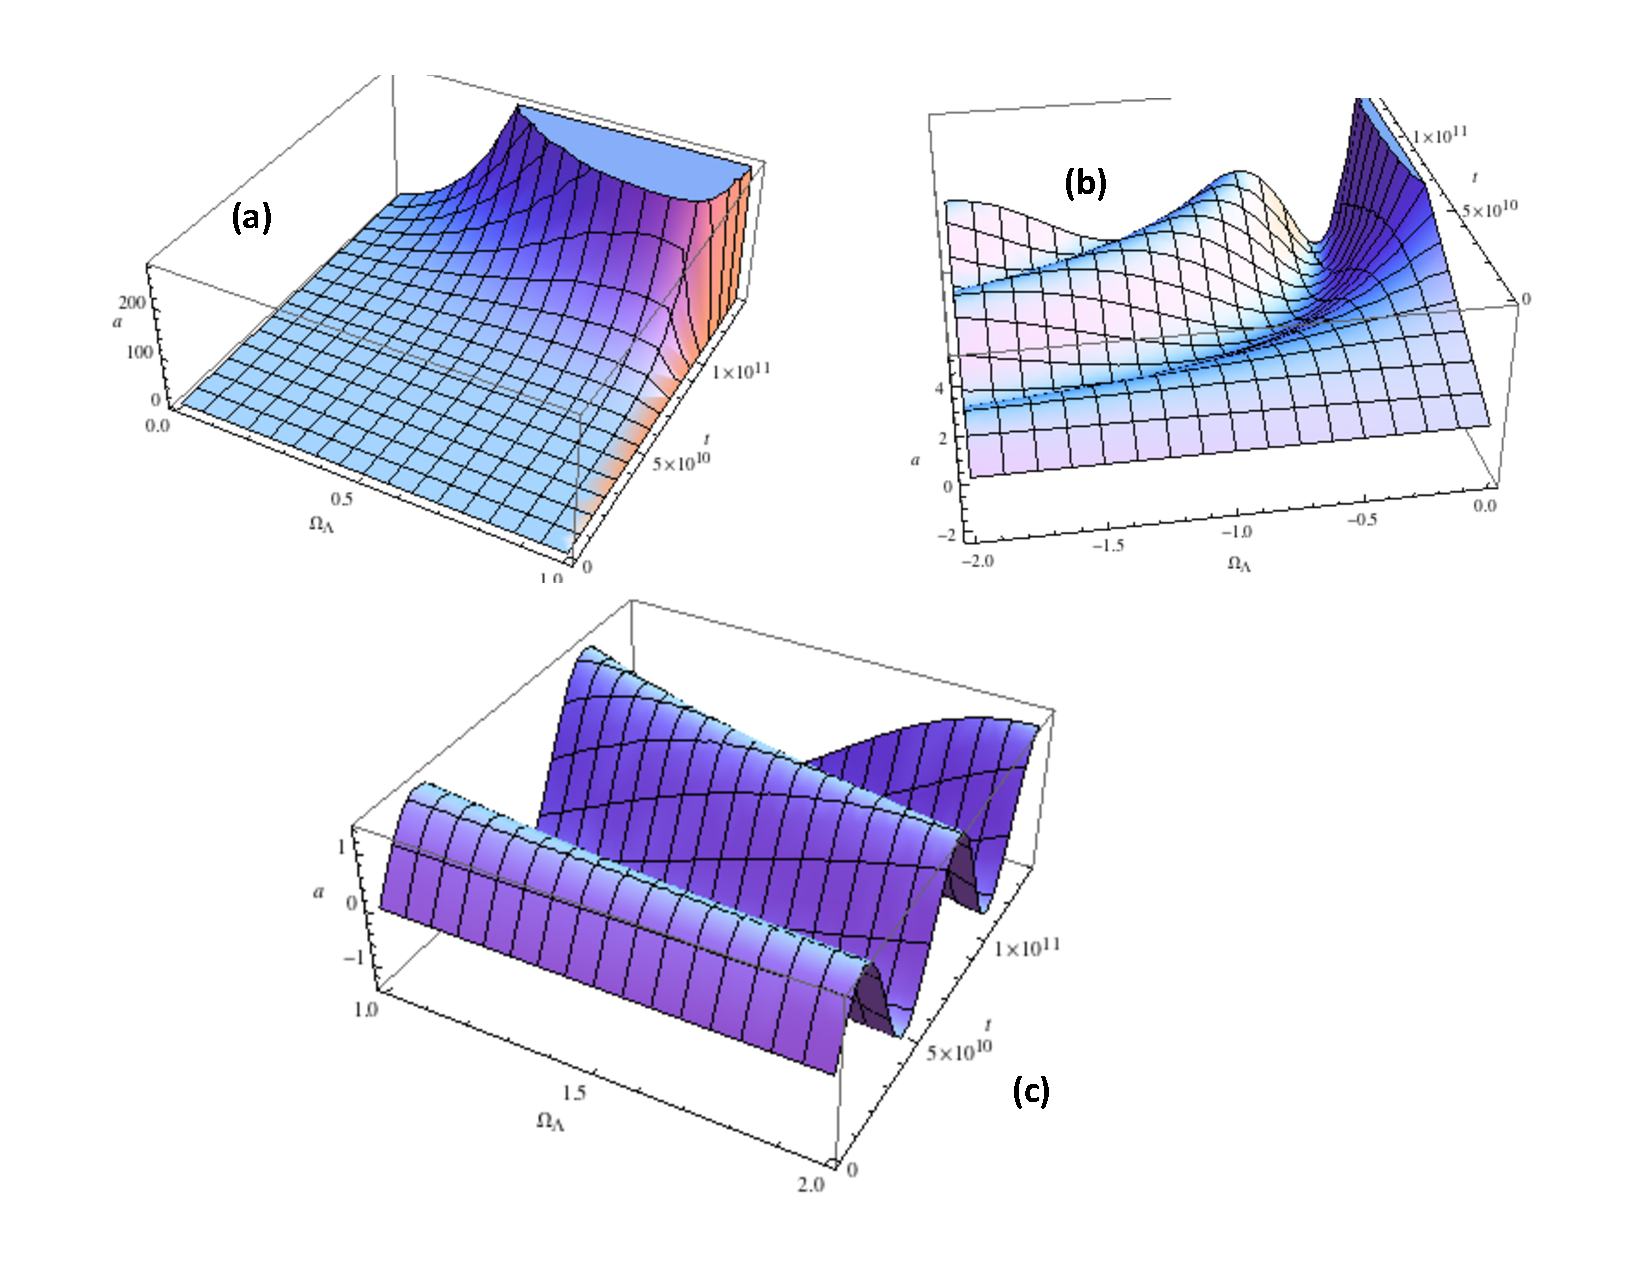
\includegraphics[width=1.2\textwidth]{aBigBang.pdf}
  \caption{The surfaces depict the behavior of the scale factor as a function of both $t$ and $\Omega_{\Lambda,0}$. (a), (b), (c) are representative of the two solution, presented in equations \ref{eq:aOfT1} and \ref{eq:aOfT2} for the 3 regions of interest: $0<\Omega_{\Lambda,0}<1$, $\Omega_{\Lambda,0}<0$, and $1<\Omega_{\Lambda,0}$ respectively.}\label{f:aOfTBigbang}
\end{figure}



%=========================================
\subsubsection{No Big Bang}
For universes without a Big Bang the only boundary condition available to us for determining the value of $C$ is the normalization of the scale factor. Recall that $a(t_{0}) = 1$.  Enforcing that condition,
\begin{align}
&1 = \frac{1}{2\Omega_{\Lambda,0}} e^{-\sqrt{\Omega_{\Lambda,0}}(H_{0}t_{0}+C)}\left(e^{2\sqrt{\Omega_{\Lambda,0}}(H_{0}t_{0}+C)}+\Omega_{\Lambda,0}(\Omega_{\Lambda,0}-1)\right)\\
&C_{\pm} = -H_{0}t_{0}+\frac{\ln\left(\Omega_{\Lambda,0}\pm\sqrt{\Omega_{\Lambda,0}}\right)}{\sqrt{\Omega_{\Lambda,0}}}
\end{align}
 Inserting these values for $C$,
\begin{align}
a(t) &= \frac{e^{-H_{0}\sqrt{\Omega_{\Lambda,0}}(t-t_{0})}}{2\sqrt{\Omega_{\Lambda,0}}}\left[e^{2H_{0}\sqrt{\Omega_{\Lambda,0}}(t-t_{0})} \left(\sqrt{\Omega_{\Lambda,0}}\pm 1\right)+\sqrt{\Omega_{\Lambda,0}}\mp 1\right]\\
 &=\Omega_{\pm}e^{H_{0}\sqrt{\Omega_{\Lambda,0}}(t-t_{0})}+\Omega_{\mp}e^{-H_{0}\sqrt{\Omega_{\Lambda,0}}(t-t_{0})}\label{eq:noBig1}
\end{align}
Where we have defined,
\begin{align}
\Omega_{\pm} = \frac{\sqrt{\Omega_{\Lambda,0}}\pm 1}{2\sqrt{\Omega_{\Lambda,0}}}\quad\&\quad \Omega_{\mp} = \frac{\sqrt{\Omega_{\Lambda,0}}\mp 1}{2\sqrt{\Omega_{\Lambda,0}}}
\end{align}

For $\Omega_{\Lambda,0}<0$ the solution is oscillatory and similar to the discussion of equation~\ref{eq:osc},
\begin{align}
a(t) = \Omega_{\pm}e^{iH_{0}\sqrt{|\Omega_{\Lambda,0}|}(t-t_{0})}+\Omega_{\mp}e^{-iH_{0}\sqrt{|\Omega_{\Lambda,0}|}(t-t_{0})} \qquad\text{\textbf{for \quad $\Omega_{\Lambda,0}<0$}}\label{eq:noBig2}
\end{align}
\textbf{Note} that we must also substitute $i\sqrt{|\Omega_{\Lambda,0}|}$ for $\sqrt{\Omega_{\Lambda,0}}$ in $\Omega_{\pm}$ and $\Omega_{\mp}$.\par

As in section~\ref{s:abigbang} figure~\ref{f:aOfTNoBigbang} depicts the relationship between $a$ and both $t$ and $\Omega_{\Lambda,0}$. Note that $t_{0}$ and $H_{0}$ have both been normalized to one and we have only chosen to depict the second solution of equations~\ref{eq:noBig1} and \ref{eq:noBig2} (i.e. $\Omega_{\pm}\rightarrow\Omega_{-}$ and $\Omega_{\mp}\rightarrow\Omega_{+}$). One can see from both  figure (a) and (c) that under particular conditions one can generate a bouncing universe, one that reaches a minimum then continues to expand forever. Figure (b) is very similar to figure~\ref{f:aOfTBigbang} (c) except that it starts at a maximum or close to a maximum then plummets down until it reaches zero. Figure (c) is a cross-section of figure (a), I chose $\Omega_{\Lambda,0} = 2$ in order to depict an example of a "Bouncing Universe."

\begin{figure}[h!]
  \centering
      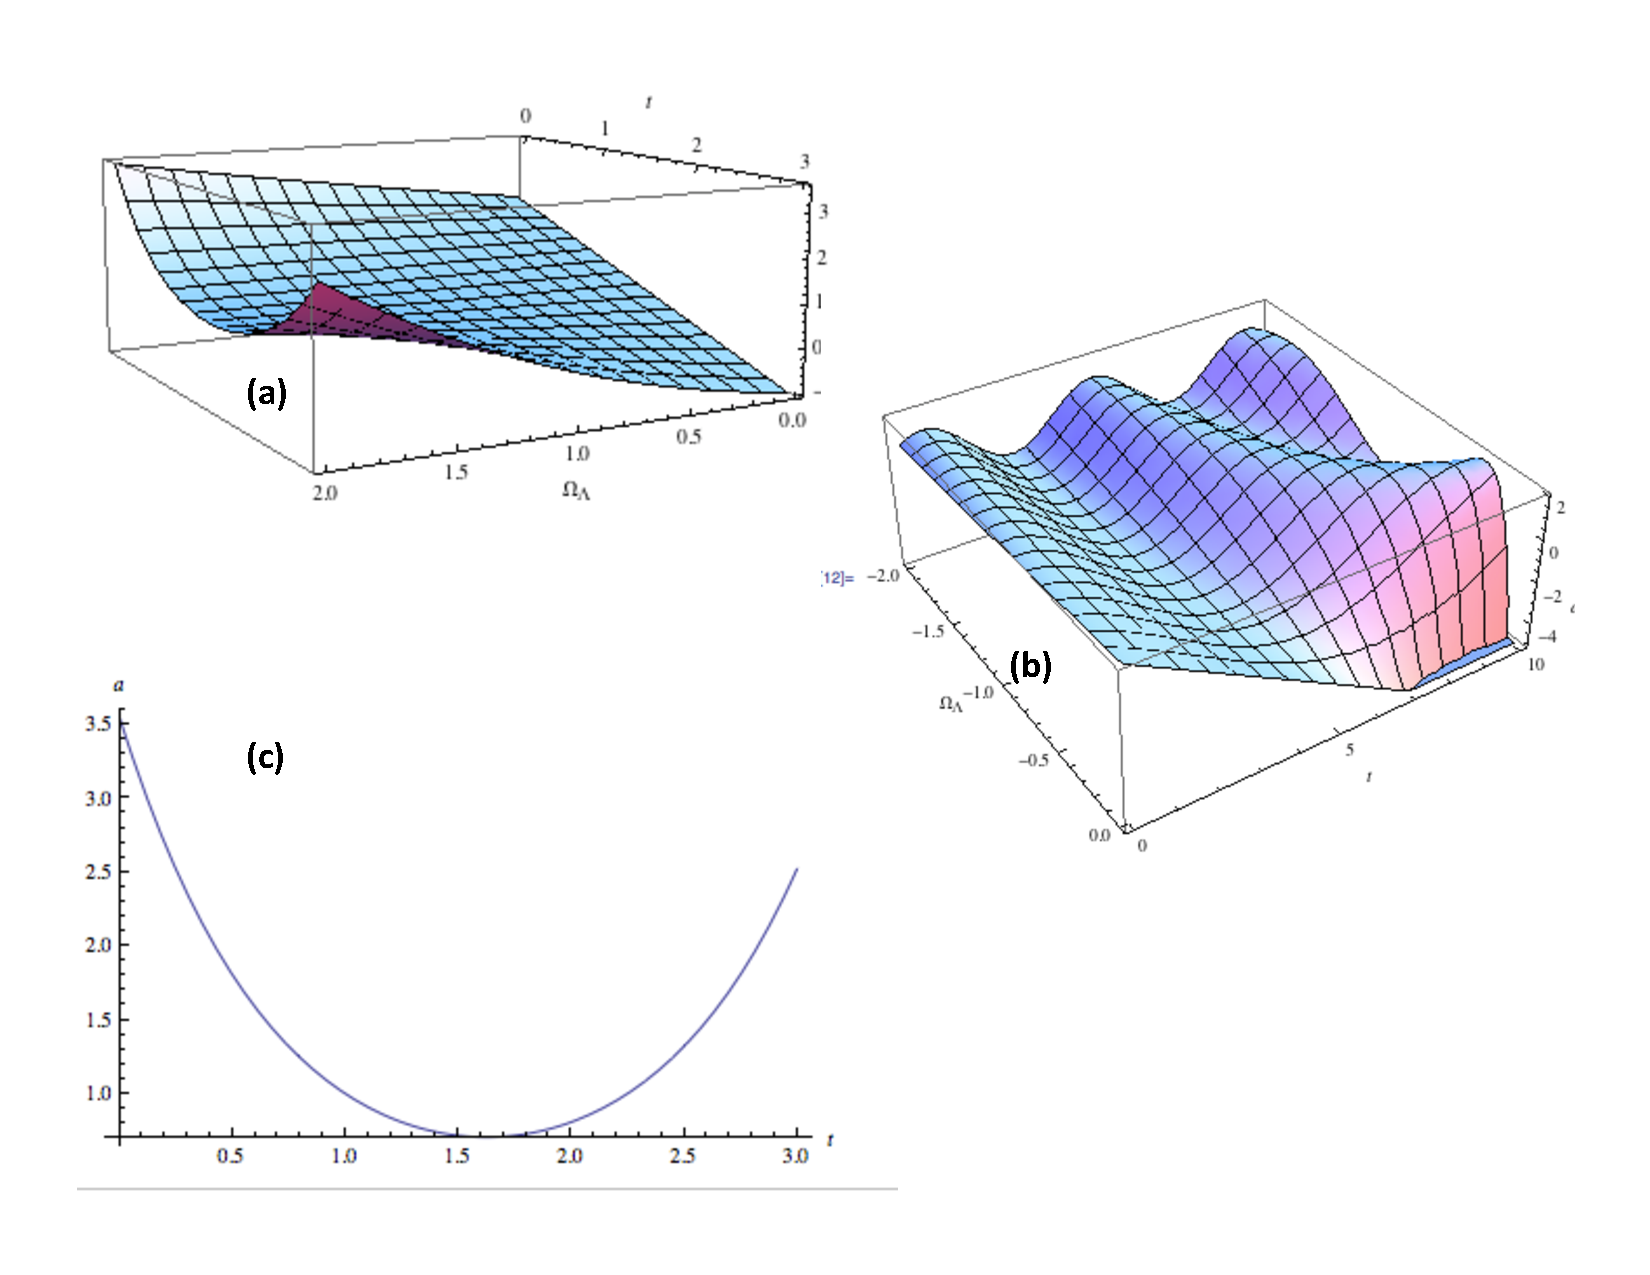
\includegraphics[width=1.2\textwidth]{aOfTNoBigBang.pdf}
  \caption{The surfaces depict the behavior of the scale factor as a function of both $t$ and $\Omega_{\Lambda,0}$. Note that $t_{0}$ and $H_{0}$ have both been normalized to one and we have only chosen to depict the second solution of equations~\ref{eq:noBig1} and \ref{eq:noBig2} (i.e. $\Omega_{\pm}\rightarrow\Omega_{-}$ and $\Omega_{\mp}\rightarrow\Omega_{+}$). (a) and (c) correspond to solution~\ref{eq:noBig1}, (b) to the other. Figure (c) is a cross-section of figure (a), I chose $\Omega_{\Lambda,0} = 2$ in order to depict an example of a "Bouncing Universe." }\label{f:aOfTNoBigbang}
\end{figure}


%=======================================
\newpage
\appendix
%=======================================
\section{Constant $\Omega_{\Lambda}$}\label{a:constOmeg}
%=======================================
We mentioned in section~\ref{s:simplify} that although $\rho_{\Lambda}$ is constant $\Omega_{\Lambda}$ is not because the critical density, $\rho_{c}$  (see equation~\ref{eq:cirtDen}), is time dependent. Yet there is a value of $\Omega_{\Lambda,0}$ that causes $\Omega_{\Lambda}$ to remain constant.\par
By definition in order for a quantity to remain constant with respect to time its time derivative must be equal to zero for all time. With this in mind,
\begin{align}
&\Omega_{\Lambda}  = \Omega_{\Lambda,0}\frac{H^{2}_{0}}{H^{2}}, \quad \text{one can show:}\label{eq:omegLamb}\\
&\dot{\Omega}_{\Lambda} = \frac{2H^{2}_{0}}{H^{3}a}(H^2a-\ddot{a})
\end{align}
Thus if we are interested in a static $\Omega_{\Lambda}$ the condition of interest is $H^{2} = \ddot{a}/a$. Noting that we are particularly interested in the case where $\Omega_{\Lambda} = \Omega_{\Lambda,0}$. From eq~\ref{eq:omegLamb}, we see that this happens when  $H^2=H_{0}^{2}$. From the condition of interest this implies that $\ddot{a}/a= H^{2}=H^{2}_{0}$, This relation is only satisfied if $H_{0}  = 0$ and $a = $ constant, meaning that the universe is and always has been static. \par

We also come to the conclusion,through the use of equation~\ref{eq:acce} ,that $\Omega_{\Lambda,0} =1$. This also implies that the universe must be flat, $k=0$. This can also be seen from table~\ref{t:signK} and equation~\ref{eq:friedmanN}, with $\Omega_{\Lambda}=\Omega_{\Lambda,0}=1$, $\Omega_{k}$ must equal 0.


%=======================================
\section{The Age of the Universe}
Because the scale factor has been normalized to be one "today" ($t_{0}$), in accordance to cosmological formalism which we have followed throughout, for universes with a big bang it is relatively straight forward to compute this time. One merely needs to invert equations~\ref{eq:aOfT1} and \ref{eq:aOfT2} to find,
\begin{align}
&t_{0} = \frac{1}{H_{0}\sqrt{\Omega_{\Lambda,0}}}\sinh^{-1}\left(\sqrt{\frac{\Omega_{\Lambda,0}}{1-\Omega_{\Lambda,0}} }\right)\quad \text{\textbf{for}}\quad 0<\Omega_{\Lambda,0}<1\\
&t_{0} = \frac{1}{H_{0}\sqrt{|\Omega_{\Lambda,0}|}}\sin^{-1}\left(\sqrt{\frac{|\Omega_{\Lambda,0}|}{1+|\Omega_{\Lambda,0}|} }\right)\quad \text{\textbf{for}}\quad \Omega_{\Lambda,0}<0\quad\&\quad \Omega_{\Lambda,0}>1
\end{align}
$t_{0}$ vs $\Omega_{\Lambda,0}$ for both cases is plotted on figure~\ref{f:t0vsOmeg}. The discontinuity at $\Omega_{\Lambda,0} = 1$ can be explained by the fact that as $\Omega_{\Lambda}\rightarrow 1$ the universe becomes static (see appendix~\ref{a:constOmeg}) and thus the age infinite; $t_{0}$ drops of quickly  as $|\Omega_{\Lambda,0}|\rightarrow\infty$. A large value of the cosmological constant indicates a large magnitude of acceleration that will reduce the time necessary to observe the values of current parameters such as $H_{0}$
\begin{figure}[h!]
  \centering
      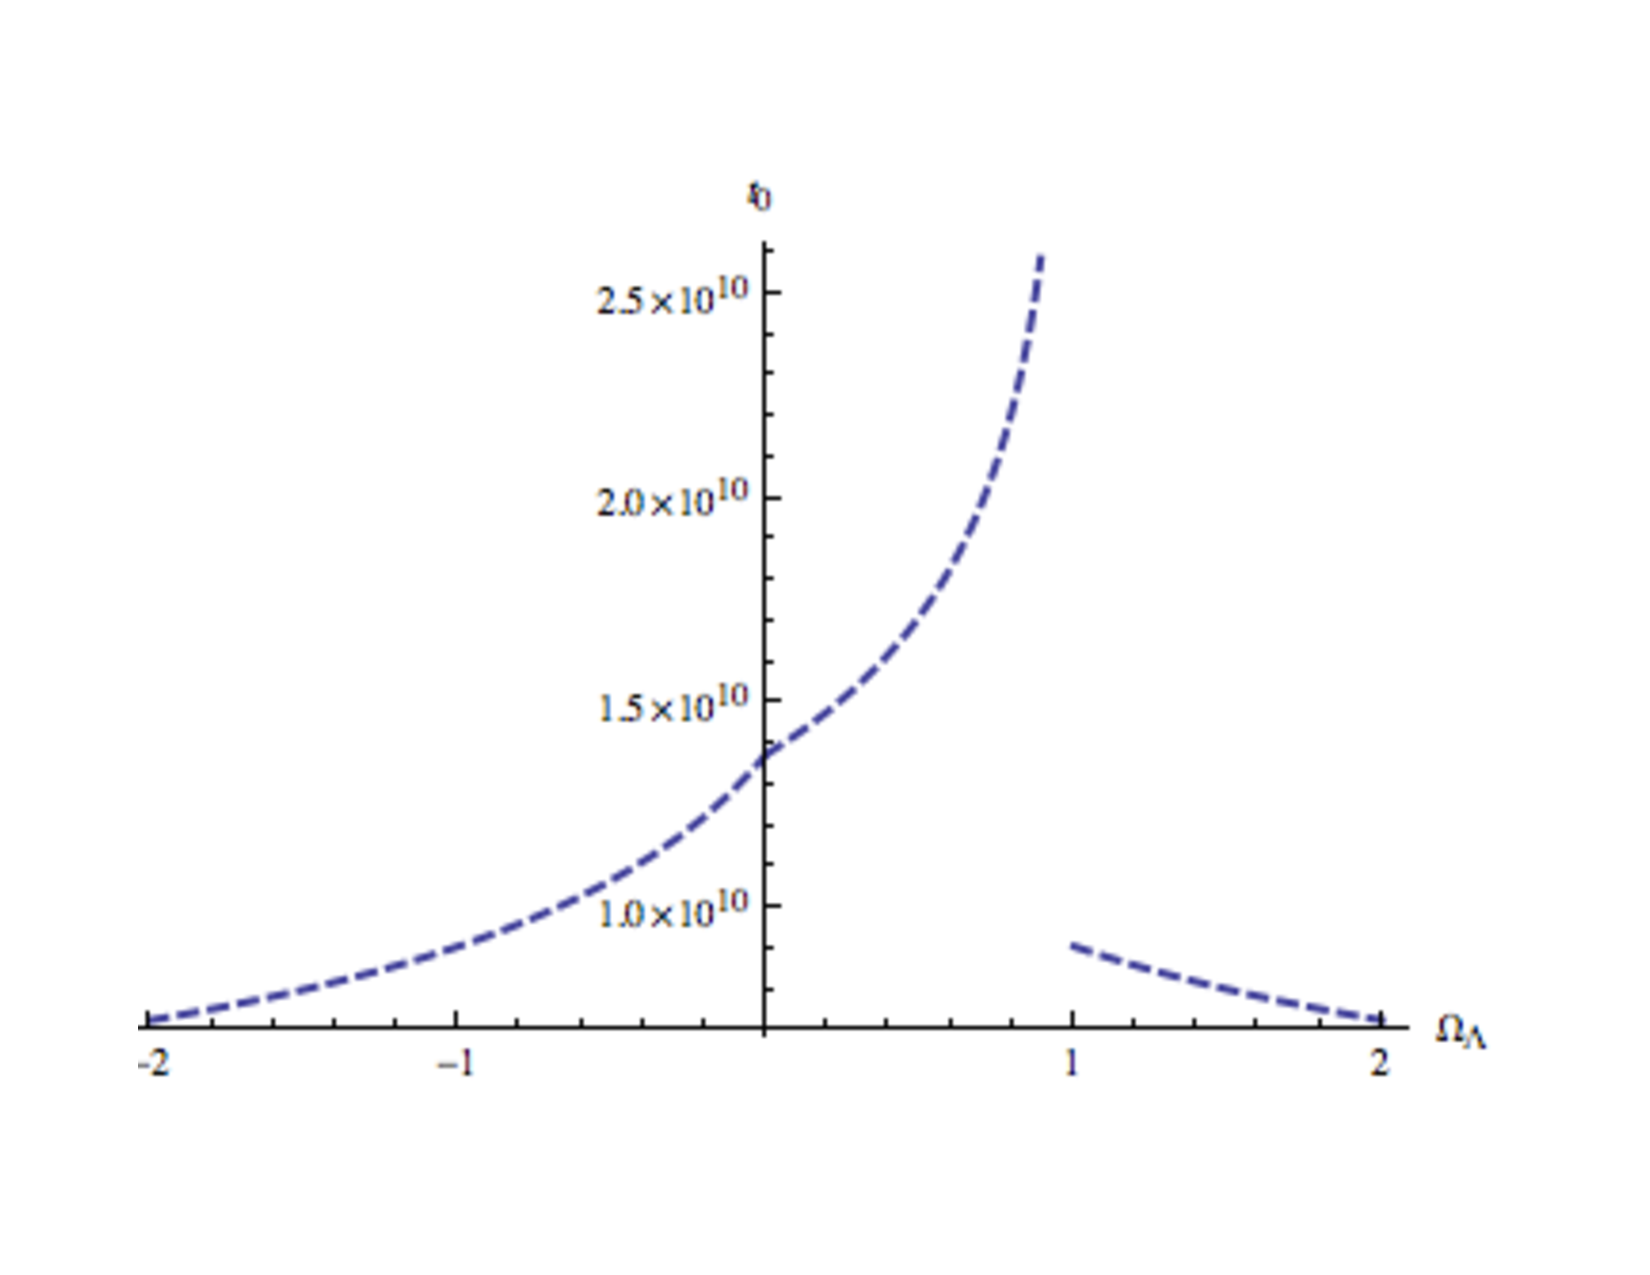
\includegraphics[width=1\textwidth]{tvsOmega.pdf}
  \caption{$t_{0}$ vs $\Omega_{\Lambda,0}$ for both positive and negative values of $\Omega_{\Lambda,0}$. Note that the value of $H_{0} = 72 [km/s\cdot Mpc]$ was used.}\label{f:t0vsOmeg}
\end{figure}

For universes without a Big Bang, the word "age" no longer has a clear meaning.  What marks the "beginning"? $t_{0}$ is now only conventionally relevant as the normalization of the scale factor "today."  It might be suitable to reference time to the local minimum of $a(t)$ but this would mean that if that local minimum is in the future we would need to speak in terms of negative time, or even a count down towards the end of the universe. 

%=======================================
\section{The Time Evolution of $\Omega_{\Lambda}$}
From equation~\ref{eq:omegLamb1} we see that $\Omega_{\Lambda}$ depends on the scale factor in the following way,
\begin{align}
\Omega_{\Lambda} = \Omega_{\Lambda,0}\frac{a^{2}(t)H^{2}_{0}}{\dot{a}^{2}}
\end{align}
Given that we have, at hand, solutions for $a(t)$  and that the derivatives of $\sinh$ and $\sin$ are $\cosh$ and $\cos$ respectively we may directly compute $\Omega_{\Lambda}$.
\begin{align}
\Omega_{\Lambda,0} = \left\{\begin{array}{ll}\tanh^{2}(H_{0}\sqrt{\Omega_{\Lambda,0}}t)\quad \text{for}\quad 0<\Omega_{\Lambda,0}<1\\\\ \tan^{2}(H_{0}\sqrt{|\Omega_{\Lambda,0}|}t)\quad \text{for}\quad \Omega_{\Lambda,0}<0\quad\&\quad\Omega_{\Lambda,0}>1 \end{array}\label{eq:omegLambT}\right\}
\end{align}
 On figure~\ref{f:OmegLamb} I have plotted the  expressions in equation~\ref{eq:omegLambT}\par

\begin{figure}[h!]
  \centering
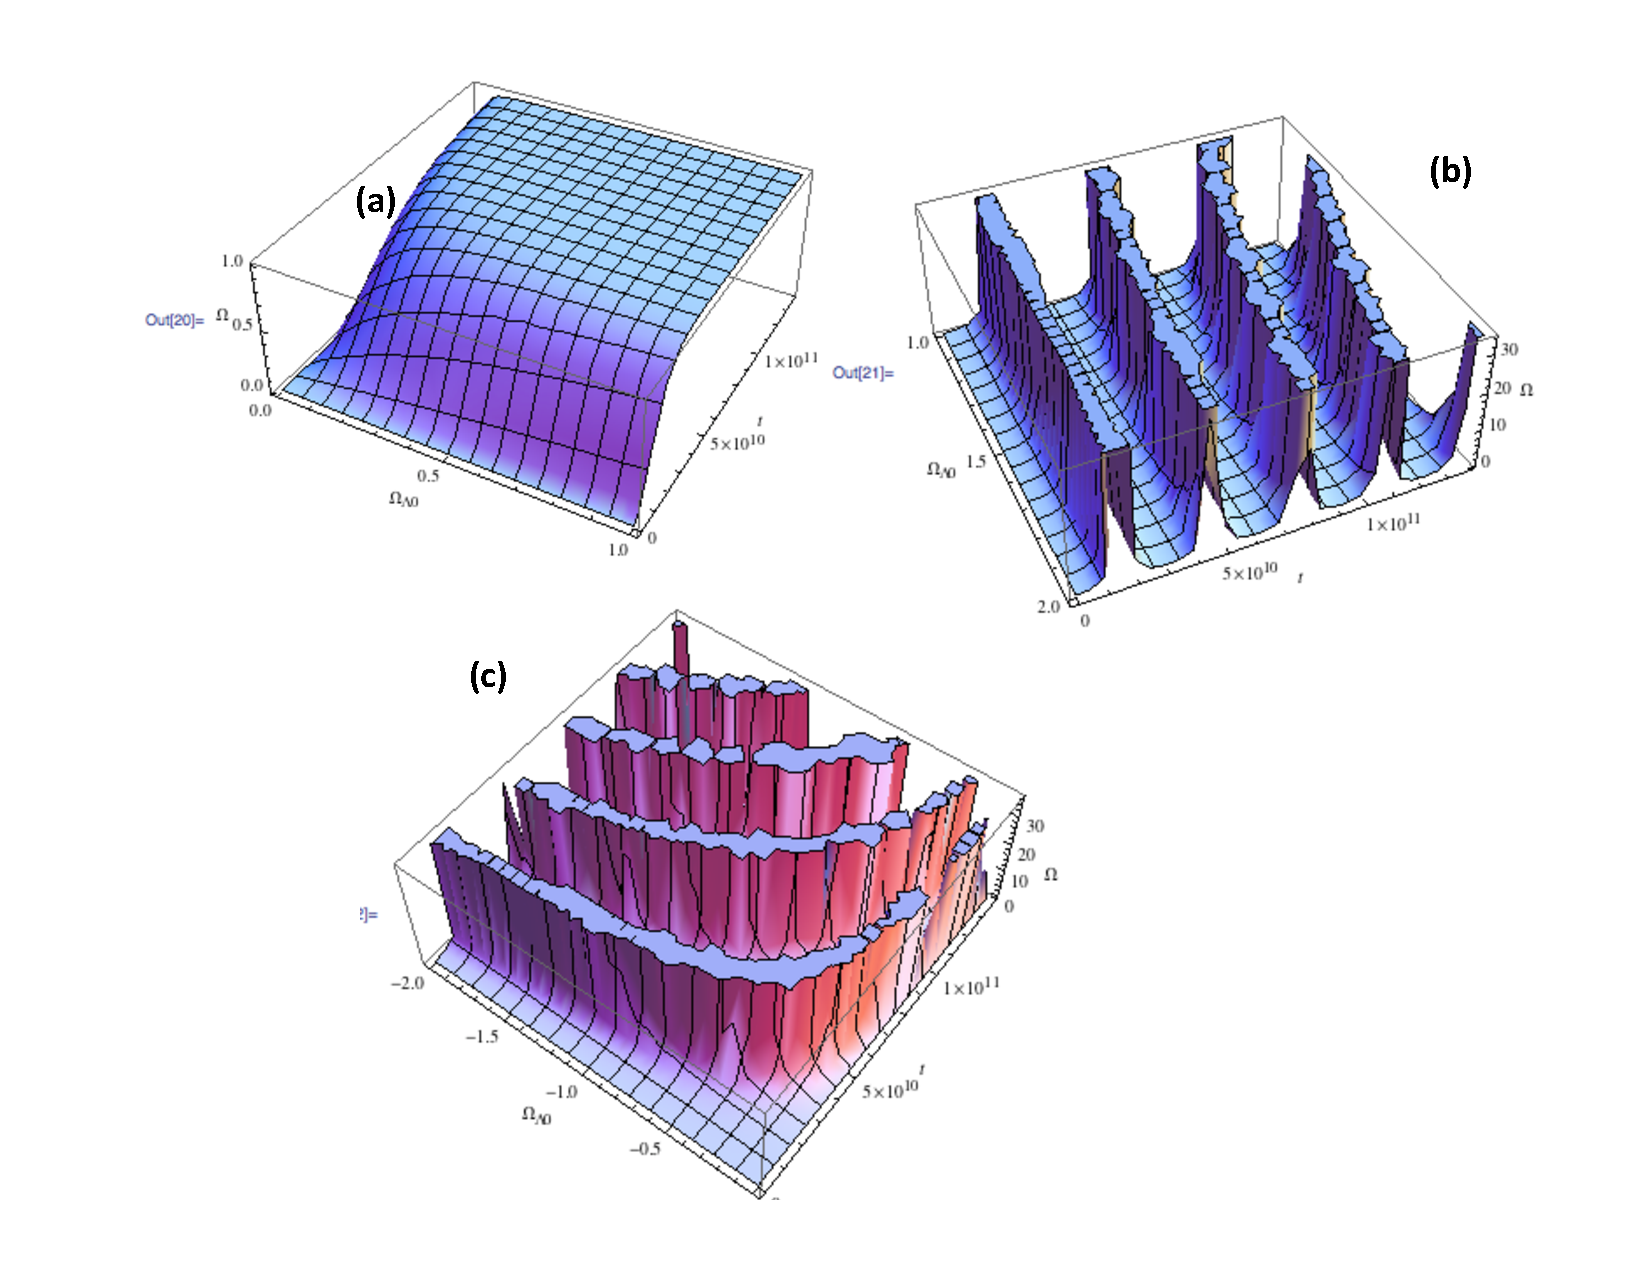
\includegraphics[width=1.2\textwidth]{OmegLamb.pdf}
  \caption{ For (a), (b), and (c) I took into consideration solutions presented in equations \ref{eq:aOfT1} and \ref{eq:aOfT2} for the 3 regions of interest: $0<\Omega_{\Lambda,0}<1$, $\Omega_{\Lambda,0}<0$, and $1<\Omega_{\Lambda,0}$ respectively. }\label{f:OmegLamb}
\end{figure}

We again note that the universe is of finite age for the regimes shown on figure~\ref{f:OmegLamb} (b) and (c). I have plotted beyond the finite age to display the general trigonometric trend. We note that for  $0<\Omega_{\Lambda,0}<1$ although the universe expands forever the value of $\Omega_{\Lambda}$ asymptotes to one implying from equation~\ref{eq:friedmanN} that the universe becomes $\Lambda$ dominated with $\Omega_{K}$ playing a negligible role.
%=======================================
%=======================================

\end{document}




%---------------------------------------------------



\begin{figure}[h!]
  \centering
      \includegraphics[width=0.5\textwidth]{gull}
  \caption{A picture of the same gull
           looking the other way!}
\end{figure}
 #==================================================


\begin{table}[h!]
  \begin{center}
    \begin{tabular}{| l c r |}
    \hline
    1 & 2 & 3 \\
    4 & 5 & 6 \\
    7 & 8 & 9 \\
    \hline
    \end{tabular}
  \end{center}
  \caption{A simple table}
\end{table}
#========================================================

\usepackage{graphicx}
\usepackage{caption}
\usepackage{subcaption}
 
\begin{figure}
        
        \begin{subfigure}[b]{0.3\textwidth}
                \centering
                \includegraphics[scale=.5]{MagVsTg.pdf}
                \caption{A gull}
                \label{fig:gull}
        \end{subfigure}%
        \hspace{3cm} %add desired spacing between images, e. g. ~, \quad, \qquad etc. 
          %(or a blank line to force the subfigure onto a new line)
        \begin{subfigure}[b]{0.3\textwidth}
                \centering
                \includegraphics[scale=.5]{MagVsTi.pdf}
                \caption{A tiger}
                \label{fig:tiger}
        \end{subfigure}
        ~ %add desired spacing between images, e. g. ~, \quad, \qquad etc. 
          %(or a blank line to force the subfigure onto a new line)
	\\
        \begin{subfigure}[b]{0.3\textwidth}
                \centering
                \includegraphics[scale=.5]{MagVsTr.pdf}
                \caption{A mouse}
                \label{fig:mouse}
        \end{subfigure}
	\hspace{3cm} %add desired spacing between images, e. g. ~, \quad, \qquad etc. 
          %(or a blank line to force the subfigure onto a new line)
        \begin{subfigure}[b]{0.3\textwidth}
                \centering
                \includegraphics[scale=.5]{MagVsTu.pdf}
                \caption{A mouse}
                \label{fig:mouse}
        \end{subfigure}
	\\
        \begin{subfigure}[b]{0.3\textwidth}
                \centering
                \includegraphics[scale=.5]{MagVsTz.pdf}
                \caption{A mouse}
                \label{fig:mouse}
        \end{subfigure}

        \caption{Absolute Magnitude Vs Time}\label{fig:animals}

\end{figure}
